\begin{frame}[parent={cmap:jabuti-gui},hasnext=true,hasprev=true]
\frametitle{Main functionalities}
\framesubtitle{Visualization Menu}
\label{concept:visualization-menu}

\begin{block}{Visualization}
The \highlight{Visualization} menu provides different forms of visualization of
the classes and methods under testing.
\end{block}

\begin{block}{Demo}
\insertmovie{resources/JaBUTi/JaBUTi-GUI/JaBUTi-GUI-Visualization/JaBUTi-GUI-Visualization}
\end{block}
\end{frame}



\begin{frame}
\frametitle{Main functionalities}
\framesubtitle{Visualization Menu}
\label{concept:current-bytecode-file}

\begin{block}{Current Bytecode File}
\highlight{Current Bytecode File} option shows the highlighted bytecode of the
currently selected class file.
\end{block}

\begin{block}{Demo}
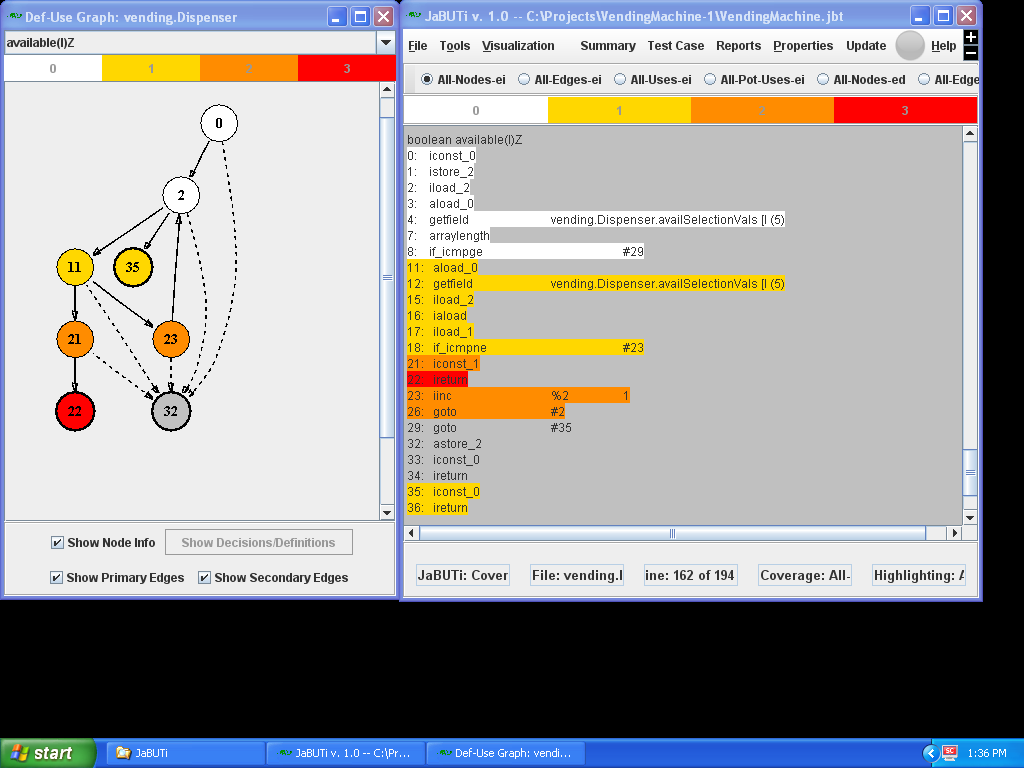
\includegraphics[width=\textwidth,clip]{resources/JaBUTi/JaBUTi-VendingMachine/JaBUTi-VendingMachine-Visualization-DugAndBytecode}
\end{block}
\end{frame}



\begin{frame}
\frametitle{Main functionalities}
\framesubtitle{Visualization Menu}
\label{concept:current-source-file}

\begin{block}{Current Source File}
\highlight{Current Source File} option shows the highlighted source
code of the current selected class file.
\end{block}

\begin{block}{Demo}
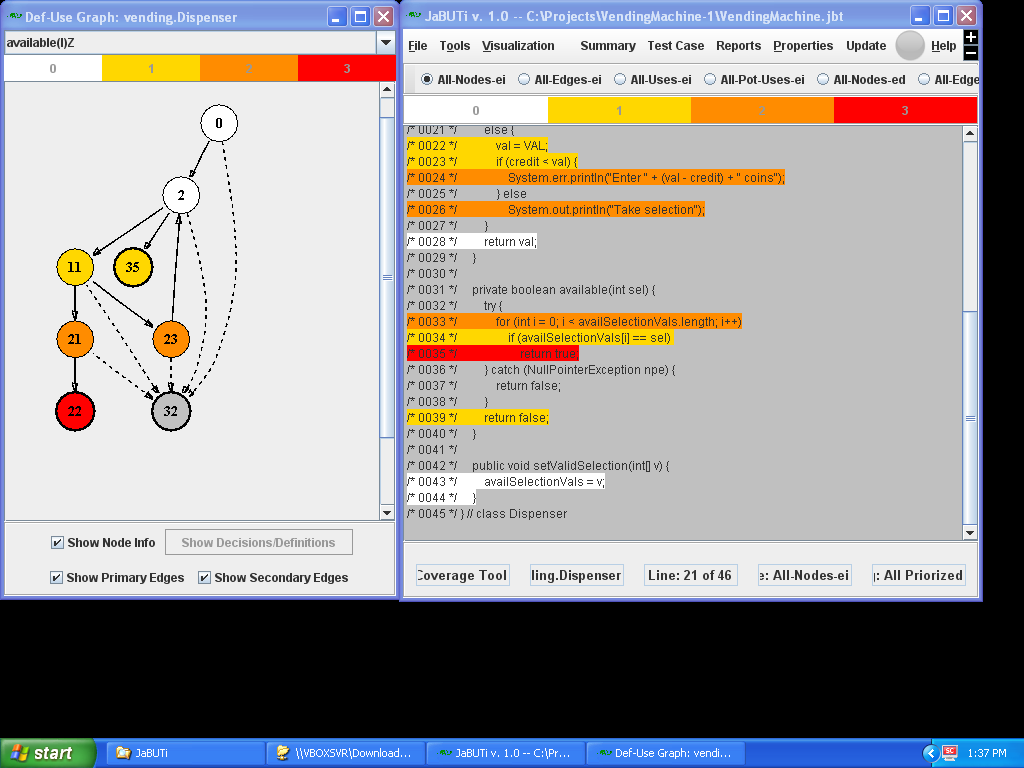
\includegraphics[width=\textwidth,clip]{resources/JaBUTi/JaBUTi-VendingMachine/JaBUTi-VendingMachine-Visualization-DugAndSourceCode}
\end{block}
\end{frame}



\begin{frame}
\frametitle{Main functionalities}
\framesubtitle{Visualization Menu}
\label{concept:required-elements}

\begin{block}{Required Elements}
\highlight{Required Elements} option shows the set of required elements for a
given method of a given class, considering the current selected criterion.
\end{block}

\begin{block}{Demo}
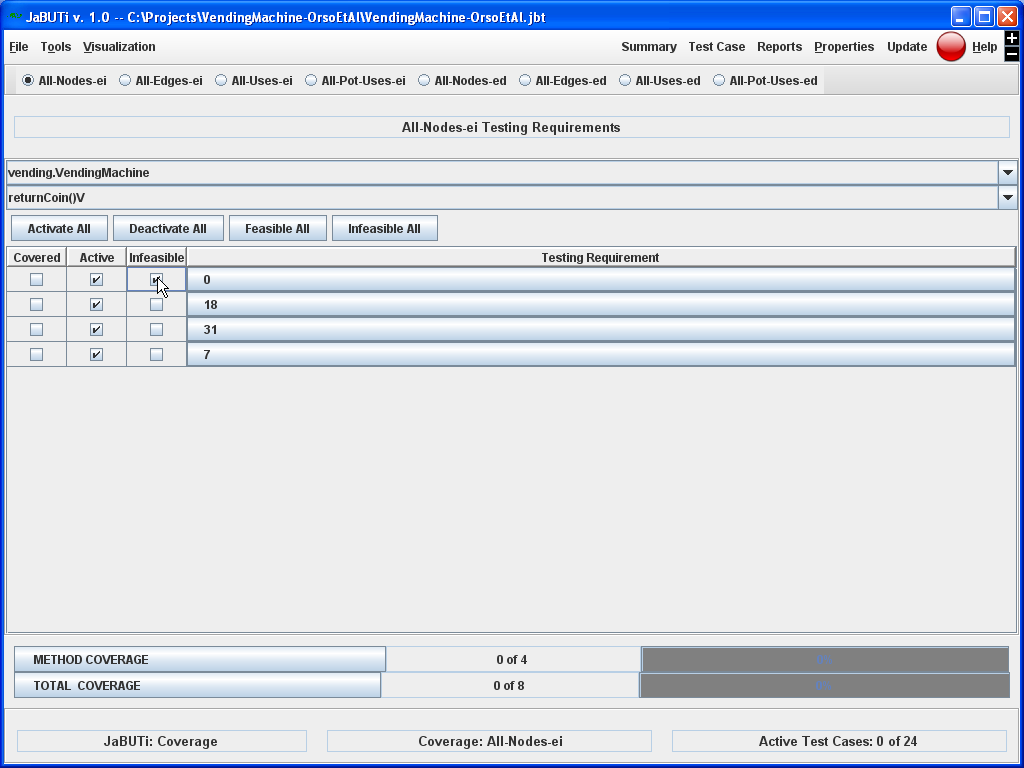
\includegraphics[width=\textwidth,clip]{resources/JaBUTi/JaBUTi-VendingMachine/JaBUTi-VendingMachine-vending.VendingMachine-TestCaseManagement}
\end{block}
\end{frame}



\begin{frame}
\frametitle{Main functionalities}
\framesubtitle{Visualization Menu}
\label{concept:def-use-graph}

\begin{block}{Def-use-graph}
\highlight{Def-Use Graph} option shows the definition-use graph of a given
method of the current class.
\end{block}

\begin{block}{Demo}
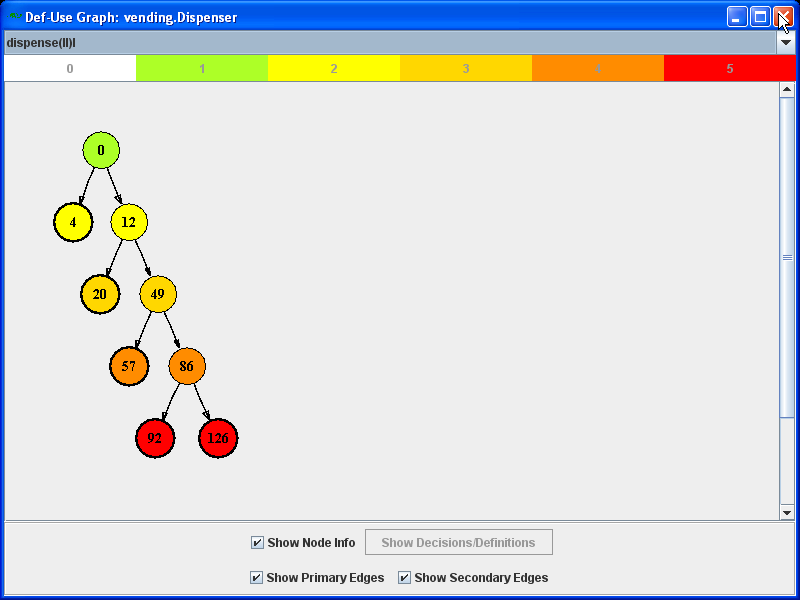
\includegraphics[width=\textwidth,clip]{resources/JaBUTi/JaBUTi-VendingMachine/JaBUTi-VendingMachine-vending.Dispenser-DUG}
\end{block}
\end{frame}



\begin{frame}
\frametitle{Main functionalities}
\framesubtitle{Visualization Menu}
\label{concept:complexity-metrics}

\begin{block}{Complexity Metrics}
\highlight{Complexity Metrics} option shows the resultant value of the set of
complexity metrics implemented in JaBUTi for the complete set of user classes
obtained from the base class (classes under testing).
\end{block}

\begin{block}{Demo}
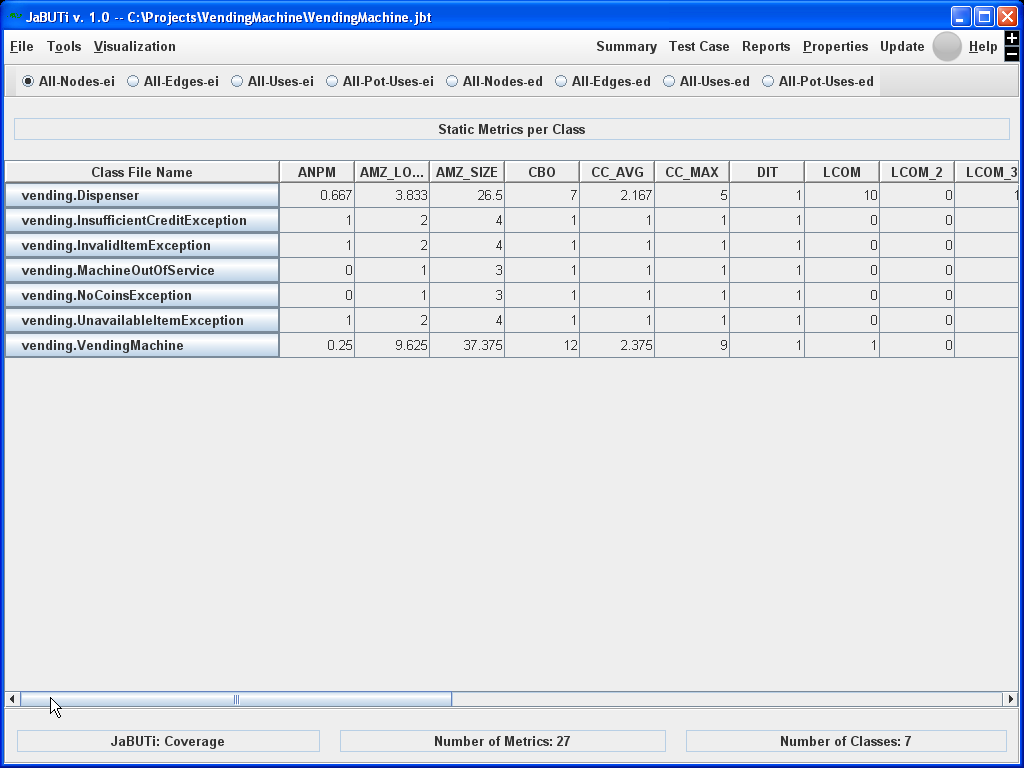
\includegraphics[width=\textwidth,clip]{resources/JaBUTi/JaBUTi-VendingMachine/JaBUTi-VendingMachine-Metrics}
\end{block}
\end{frame}